\section{Auswertung}
\label{sec:Auswertung}

\begin{figure}
  \centering
  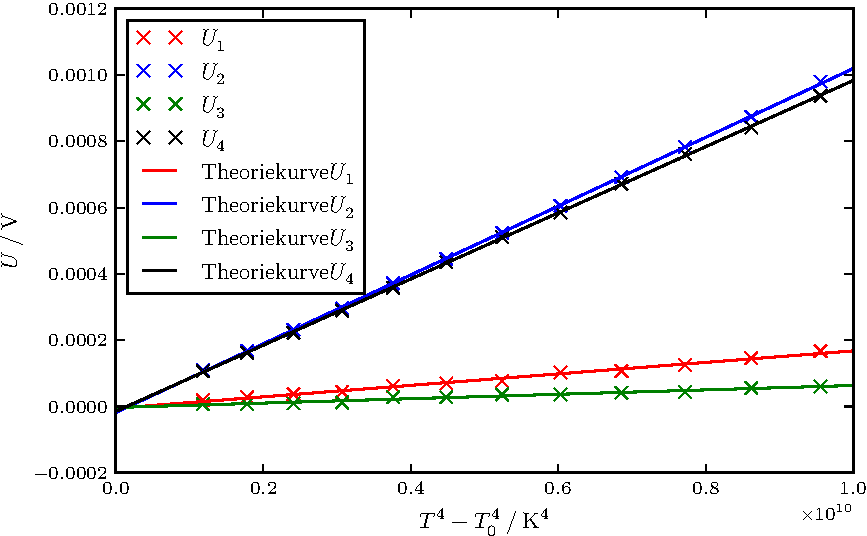
\includegraphics{plot.pdf}
  \caption{Plot.}
  \label{fig:plot}
\end{figure}


%\begin{table}
%  \centering
%  \caption{Beispieltabelle}
%  \label{tab:tabelle_beispiel}
%  \sisetup{table-format=1.2}
%  \begin{tabular}{c c}
%    \toprule
%    {$a [\si{\second}]$} & {$b [\si{\kelvin}]$}\\
%    \midrule
%    1.0000  & 11.00 \\
2.0000  & 12.00 \\
3.0000  & 13.00 \\
4.0000  & 14.00 \\
5.0000  & 15.00 \\
6.0000  & 16.00 \\
7.0000  & 17.00 \\
8.0000  & 18.00 \\
9.0000  & 19.00 \\
10.0000 & 20.00 \\

%    \bottomrule
%  \end{tabular}
%\end{table}
%
%Es ergibt sich
%\begin{align}
%  a &= (0 \pm 0) ~ \si{\joule\per\kelvin\per\gram}
 \\
%\end{align}

\subsection{RC-Glied zur Integration}
Das RC-Glied wird, wie in der Durchführung beschrieben, zur Integration der angelegten Spannung genutzt.
Dabei wird eine Frequenz von $\nu = \SI{3000}{\hertz}$ verwendet.
Zunächst wird eine Sinusspannung angelegt, so dass
\begin{align}
U_G &= U_0\sin{\omega t}  & U_c &= -\frac{U_0}{\omega}\cos{\omega t}
\end{align}
als Spannungen erwartet werden, wobei $U_G$ die angelegte Spannung, $U_c$ die erwartete Kondensatorspannung und $U_0$ die Amplitude der Sinusspannung bezeichnet.
In Abbildung \ref{fig:sin_s} wird schematisch das erwartete Ergebnis , in \ref{fig:sin_r} das am Oszillographen abgelesene Ergebnis abgebildet.

% Insert Pics here

Als nächstes wird die Rechteckspannung überprüft, so dass die Werte
\begin{align}
  U_G &=
  \begin{cases}
    U_0 , &  0 \leq t \leq \frac{T}{2} \\
    -U_0 , & \frac{T}{2} \leq t \leq T
  \end{cases}
   & U_c &=
  \begin{cases}
    at , &  0 \leq t \leq \frac{T}{2} \\
    -at , & \frac{T}{2} \leq t \leq T
  \end{cases}
\end{align}
mit $U_0$ als Amplitude der Rechteckspannung sowie $a$ als positiven Skalierungsfaktor erwartet werden.
Abbildung \ref{fig:rechteck_s} und \ref{fig:rechteck_r} vergleichen widerum das theoretisch zu erwartene mit dem erhaltenen Bild.

Zum Schluss wird die Sägezahnspannung überprüft, woraus sich die erwarteten Werte
\begin{align}
  U_G &=
  \begin{cases}
    at , &  0 \leq t \leq \frac{T}{2} \\
    -at , & \frac{T}{2} \leq t \leq T
  \end{cases}
  & U_c &=
  \begin{cases}
    b t^2 , &  0 \leq t \leq \frac{T}{2} \\
    -b t^2 , & \frac{T}{2} \leq t \leq T
  \end{cases}
\end{align}
mit Skalierungsfaktoren $a$ und $b$ ergeben.
Abbildung \ref{fig:sin_s} und Abbildung \ref{fig:sin_r} zeigt die erwarteten und gemessenen Bilder.
